% !TEX root = _individual/introduction.tex

%%%%%%%%%%%%%%%%%%%%%%%%%%%%%%%%%%%%%%%%%%%%%%%%%%%%%%%%%%%%%%%%%%%%%%%%%%%%%%%%
\chapter{Introduction}\label{chap:introduction}
%%%%%%%%%%%%%%%%%%%%%%%%%%%%%%%%%%%%%%%%%%%%%%%%%%%%%%%%%%%%%%%%%%%%%%%%%%%%%%%%

Nuclear engineering is the field that develops tools to harness the power of the
atomic nucleus and high-energy radiation related to it. It encompasses such
disparate areas as plasma physics, radiation detection, nuclear reactor design,
and atomic particle transport. The latter area is the study of how
statistically large numbers of fundamental particles interact with (and are
``transported'' through) matter; this
phenomena accounts for the behavior of neutrons in a nuclear reactor,
gamma rays in shielding applications, electrons in cancer therapy, and photons
in radiative transfer problems. This thesis is concerned with a
particular regime of radiative transfer known as thermal radiative transfer
(TRT).

The difficulty, expense, and impracticality of performing physical
experiments in many fields has produced a tremendous drive to cheaply
simulate physics. In conjunction with the exponentially
increasing power and exponentially decreasing cost of computers,
this has led to the rise of computational methods development:
researching and implementing accurate, practical approximations to the physical
equations that describe reality. Our work is in the field of computational
particle transport, and our goal is to develop a new, accurate, inexpensive
approximation to the equations of thermal radiative transfer.

One recent advance in methods development is the anisotropic diffusion (AD)
approximation, recently used to model steady-state neutron transport for
nuclear reactor analysis, viz.~a very high temperature reactor
(VHTR) mock-up \cite{Lar2009c,Tra2011}, for which AD showed very promising
results. The AD
method was also independently formulated for steady-state photon transport
\cite{Mor2007}, but it was not numerically tested.
Both derivations assumed an infinite medium operating at steady state.
Those two assumptions rarely hold for TRT problems, which typically change
rapidly as a
function of time and necessarily operate in a finite space. In the new
work presented here, we derive a complete theory describing anisotropic
diffusion for time-dependent transport problems in finite media. Furthermore,
the new derivation framework allows the development of other ``anisotropic''
approximations. One new member of this family is what we call the anisotropic
$P_1$ method, which is presented in this thesis.

Although the theory is developed for a general three-dimensional (3-D) space,
true 3-D simulations are expensive because of the expansive problem phase
space: the transport equations operate in three spatial coordinates $(x,y,z)$,
two angular coordinates $(\mu,\theta)$, and time $t$. Even two-dimensional (2-D)
problems, which model a system invariant in the $z$ direction, operate in the
space $(x,y,\mu,\theta,t)$. A ``toy'' geometry called \emph{flatland}
\cite{Abb1884}, recently used in methods development \cite{Asa2008,Lar2009c},
reduces the phase space to $(x,y,\theta,t)$ by constraining particles to a
two-dimensional plane. Flatland retains the complexity of multi-dimensional
space while decreasing the computational burden. A notable part of this thesis
is the investigation and application of flatland to transport methods
development.

To verify the accuracy of the newly developed anisotropic theory, we need to
compare its performance and accuracy against that of existing, proven methods.
Therefore, we compare the AD method against its competitors in several numerical
experiments, most of them using flatland geometry. Due to the complexity of
the thermal radiative transfer process, we first test individual aspects of the
theory. In particular, we verify the predicted boundary conditions in several
steady-state flatland problems \cite{Joh2011a}, and we test the time-dependent
behavior in ``linear'' radiation transport problems, which omit the nonlinear
material--radiation coupling of TRT.

Finally, we apply the new AD approximations to thermal radiative transfer
problems. We begin by comparing the performance of the new methods using
one-dimensional problems in the literature \cite{Rau2005}, and variations
thereof. The primary comparison, though, is a flatland simulation
\cite{Joh2011} inspired by a particular TRT experiment---%
the behavior of a laser-driven shock wave in a small tube filled with xenon
gas---%
in the Center for Radiative Shock Hydrodynamics (CRASH) program
\cite{Crash2010}. In addition to the flatland problems, we test some difficult
two-dimensional problems \cite{Mou2006}.

%This thesis extends a steady-state, infinite-medium anisotropic diffusion (AD)
%approximation \cite{Mor2007,Lar2009c} using a systematic derivation from the
%transport equation that accounts for time-dependent behavior and arbitrary
%problem boundaries. Our motivation is to formulate and test an approximation to
%thermal radiative transfer (TRT) that is more accurate than diffusion yet much
%less expensive than a time-dependent transport calculation.

%%%%%%%%%%%%%%%%%%%%%%%%%%%%%%%%%%%%%%%%%%%%%%%%%%%%%%%%%%%%%%%%%%%%%%%%%%%%%%%%
\section{Thermal radiative transfer}

As alluded to earlier, thermal radiative transfer models the behavior of
energy-transferring photons in hot materials. Radiation is the primary means of
heat transfer in a number of relevant physical problems such as stellar
astrophysics and fusion experiments. These systems operate at the extreme
temperatures necessary to apply the TRT model used in this thesis.

Engineering students know from their heat transfer classes that conduction and
convection transfer energy proportionally to the material
temperature $T$, but radiative energy transfer via black-body emission is
proportional to $T^4$. Thus, when $T$ is very large, conduction and convection
can be neglected. Several other reasonable assumptions reduce the phenomena of
TRT to the coupling of two variables: the space- and time-dependent material
temperature $T$, and the radiation intensity $I$.

The intensity $I$, analogous to the ``angular flux'' in the reactor physics
world,
describes the state and distribution of photons in space $\vec{x}$, angle
$\vec{\Omega}$, and time $t$%
\footnote{In this discussion, we ignore the frequency-dependent nature of light,
because the AD approximation is more suitable to gray radiation treatment than
multigroup.
}. The spatial and temporal variables are self-explanatory; the angular
variable essentially determines a photon's velocity${}=c\vec{\Omega}$, using
the speed of light $c$. More photons headed in a certain direction at a certain
point in space-time give rise to a larger value in the intensity---%
an example (outside of TRT) could be an ``intense'' flashlight being shone in
one's eyes.  The time-dependent behavior of the intensity is described by the
Boltzmann transport equation \cite{Dud1976}, sometimes referred to in the
astrophysics literature as the transfer equation \cite{Mih1984}.
The transport equation will be discussed in further detail later.

The second quantity, the material temperature $T$, is a measure of the amount
of energy stored in the atoms and electrons in the problem. When an electron
absorbs a photon, the material energy increases by exactly the amount that the
radiation intensity lost by the absorption event. As the material emits a
photon via the black body process, the lost material energy is transferred to
the radiation field.

The absorption of photons by the material, the black body emission process, and
the straight-line travel of ``streaming'' photons constitute the essence of the
thermal radiative transfer process. The rate of absorption of photons is
proportional to the opacity $\sigma$, analogous to the neutron cross section in
reactor physics. Unlike the neutron cross section, the value of $\sigma$ is
a very strong function of the material temperature.

In addition to the raw difficulty inherent in the partial differential
nature of the transport equation, the nonlinearity in $\sigma$ and in $T^4$
black body emission make the set of TRT equations more formidable than even
neutron transport. Analytically solving the TRT equations even in the
simplest problems is nearly impossible, hence the need for numerical solutions.

%%%%%%%%%%%%%%%%%%%%%%%%%%%%%%%%%%%%%%%%%%%%%%%%%%%%%%%%%%%%%%%%%%%%%%%%%%%%%%%%
\section{Overview of TRT solution methods}

Numerically solving the TRT equations is far from trivial.  The equations have
a large solution phase space and are strongly nonlinear; thus,
they are difficult to solve accurately and quickly.

TODO FROM THIS POINT ON

The past fifty years in which computers have been used to simulate radiative
transfer problems \cite{Cam1964,Cam1969} have seen major
advancements in computer technology.
Yet even today, with the need for increasingly accurate simulation of
increasingly
large and complex problems, computational power is still a limiting factor.
This is especially true in the burgeoning field of uncertainty quantification
(UQ), where many computer simulations are needed to gauge the
accuracy of the solution of a single problem.

It is one such problem in particular that inspired this work. The Center for
Radiative Shock Hydrodynamics (CRASH) program \cite{Crash2010} has the goal of
computationally predicting the behavior of a laser-driven shock in a
xenon-filled tube and providing ``error bars'' for that prediction. The accurate
simulation of energy traveling down a hollow pipe, via the process of
radiative transfer, is critical to modeling that problem. Several of the
numerical test problems in this thesis are based loosely on the CRASH problem.

Existing approximations to TRT, represented qualitatively in
Fig.~\ref{fig:fidelity}, tend to be either accurate or fast. On
the one hand are the full transport methods: Fleck and Cummings' Implicit Monte
Carlo (IMC) method \cite{Fle1971} and the discrete ordinates (\SN) method
\cite{Ada1998a}, both of which require significant time and large amounts of
computer memory. On the other hand are coarse approximations such as the
flux-limited diffusion (FLD) method \cite{Ols2000}, which makes a severe
approximation to the transport equation that yields a set of relatively simple
low-order equations. By developing a
time-dependent anisotropic diffusion approximation, we hope to provide a
\emph{via media}, where a mild increase in run time is exchanged for a
significant increase in
accuracy. The AD method could then be applied to the CRASH project or
other TRT problems to yield
realistic results in a realistic amount of time.

\begin{figure}[htb]
  \centering
  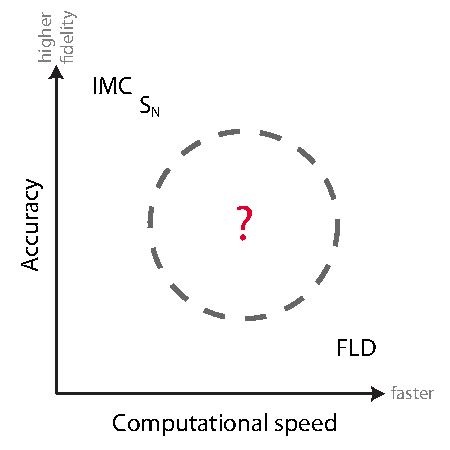
\includegraphics[width=3in]{fidelity}
  \caption{Figurative representation of existing TRT methods, showing the
  trade-off between accuracy and speed.}
  \label{fig:fidelity}
\end{figure}

%%%%%%%%%%%%%%%%%%%%%%%%%%%%%%%%%%%%%%%%%%%%%%%%%%%%%%%%%%%%%%%%%%%%%%%%%%%%%%%%
\section{Radiative transfer and anisotropic diffusion}
We begin by making some approximations to the radiative transfer
process that are common in methods development. By
\textsl{(i)} averaging over energy to get a ``gray'' (monoenergetic) radiation
intensity,
\textsl{(ii)} assuming that the material is at local thermodynamic equilibrium,
and
\textsl{(iii)} neglecting material conduction and advection,
we get a time-dependent radiation transport equation coupled to a single
material energy equation. The coupling process is the nonlinear Planckian
absorption and isotropic emission of photons: the hotter a material, the more
photons it emits.  Because the ``opacity'' of the material---%
the probability of a photon being absorbed during its flight---%
also depends on material temperature, colder materials tend to be more opaque,
or optically thick. The evolution of a system through time tends to show the
problem equilibrating by the progressive deposition of energy within a few mean
free paths of a hot region.

The anisotropic diffusion derivation starts by considering the radiation
transport equation over a time step. Rather than
making the simple diffusion approximation that the radiation intensity $I$ is a
linear function of angle, we use an integral transport equation in a novel way.
By making certain assumptions about how slowly the solution changes in space
and time, we can approximate the integral equation's nonlocal unknowns
with local unknowns. Massaging the result gives a set of low-order tensor
diffusion equations, where the AD tensor is calculated from a simple transport
equation that falls out of the analysis. Because the AD method retains a more
complicated representation of the radiation's angular behavior, we expect it
to give more accurate answers over a wide range of problems, especially those
where diffusion fails.

%Previous work \cite{Lar2009c} with the AD approximation showed very promising
%results in a steady-state Very High Temperature Reactor (VHTR) simulation;
%qualitatively, it showed how the anisotropic diffusion tensor allows particles
%to preferentially diffuse along a voided channel rather than acro

%%%%%%%%%%%%%%%%%%%%%%%%%%%%%%%%%%%%%%%%%%%%%%%%%%%%%%%%%%%%%%%%%%%%%%%%%%%%%%%%
\section{Contribution of this work}

Derivation is only a part of developing a new method: it is also
crucial to run realistic numerical experiments that help determine the method's
efficiency and efficacy. This necessitates implementing not only the new method
but also its competitors. We have implemented
diffusion, FLD, \Pone, \SN, and IMC in the \pytrt\ code \cite{Pytrt}, freely
available to the public.

As mentioned, the phase space for TRT is very large: the radiation intensity
$I$ is a function of space $\vec{x}$, angle $\vec{\Omega}$, and time $t$;
the material temperature $T(\vec{x},t)$ is also a time- and space-dependent
quantity. Recently, a fictional ``flatland'' geometry has been successfully
used as a test
bed for new methods \cite{Lar2009c,Joh2011,Tra2011}. By restricting the travel
of particles to a two-dimensional plane, one angular variable is eliminated,
yet the complexity of multi-dimensional transport is retained. The
reduced solution phase space corresponds to a reduction in computer run time:
for Monte Carlo transport, the same number of particles yields a smaller
variance in the solution, and the \SN\ method requires fewer ordinates in the
quadrature set. Thus, we use flatland geometry for the majority of our test
problems.
Our extensive use of flatland has brought to light some
interesting peculiarities of the geometry \cite{Joh2011a}; these ancillary
results are presented in this thesis.

In addition to flatland problems, we also examine the performance of the AD
method in one-dimensional and two-dimensional problems seen in the
literature. These give insight into how well AD performs in a wider variety of
situations.

%%%%%%%%%%%%%%%%%%%%%%%%%%%%%%%%%%%%%%%%%%%%%%%%%%%%%%%%%%%%%%%%%%%%%%%%%%%%%%%%
\section{Synopsis}

The remainder of this thesis is organized into the following chapters.

\chaptersynopsis{chap:trtBackground}
The assertions about the difficulty of computational modelling of thermal
radiative transfer are bolstered by presenting the equations themselves. We give
a brief overview of existing approximations to the TRT equations and discuss how
those approximations are used in our work. Particular emphasis is given to the
semi-implicit treatment, which allows the nonlinear problem to be approximated
by a system of linear equations.

\chaptersynopsis{chap:adDerivation}
With the transport equation in hand, we derive a new approximation to radiation
transport, anisotropic diffusion. The derivation accounts for both time
dependence and boundary conditions. We then discuss some of the properties of
the AD method and make predictions for its range of applicability.

\chaptersynopsis{chap:aponeDerivation}
The derivation for the time-dependent AD equations assumed that the solution
changes very slowly in time, which can be a poor approximation when applied to
TRT: it can lead to the nonphysical transfer of energy faster than the speed of
light. This chapter addresses that shortcoming in two very different ways. The
first is to apply the physically motivated but \emph{ad hoc} method of flux
limiting to the AD formulation. The second is to modify the ansatz used in
deriving the anisotropic diffusion equations, leading to a new ``anisotropic
\Pone'' method.

\chaptersynopsis{chap:implementation}
The leakage terms for anisotropic diffusion are more complex than standard
diffusion: rather than a scalar diffusion coefficient, AD has a diffusion
tensor. This necessitates unusual discretization schemes in all but the simplest
of problems. We present new discretization schemes for Cartesian \xy\ geometry
that can account for the transverse leakage induced by the anisotropic diffusion
tensor.

\chaptersynopsis{chap:flatland}
As mentioned earlier, the ``flatland'' geometry has recently proven to be a
valuable test bed for new transport methods because of its smaller phase space
and correspondingly easier solution. This chapter gives a thorough overview of
the differences between flatland and true 3-D geometries, with a focus on
implementing flatland solvers. We also explore diffusion in flatland, not only
deriving the prior result that the diffusion coefficient is different but also
formulating correct diffusion boundary conditions. Finally, we present the AD
equations in flatland geometry.

\chaptersynopsis{chap:simpleNumericalResults}
Before applying the anisotropic approximations to full nonlinear transport in
multi-dimensional geometries, it is important that we test individual components
of the derivation. We detail several steady-state problems that test the
discretization schemes, flatland diffusion boundary conditions, and anisotropic
diffusion boundary conditions. We also test some simple, linear transport
problems.

\chaptersynopsis{chap:trtNumericalResults}
Finally, we test the applicability of the anisotropic methods to the nonlinear
TRT equations. To begin, we examine a few simple 1-D test problems, where the
anisotropic methods merely ``smear'' the diffusion coefficients spatially. Then
we move to more complicated flatland problems that simulate radiation flow
through an optically thin channel. (This is the qualitative configuration of
the CRASH problem.)
Additionally, we apply the AD method to some difficult 2-D problems in the
literature that feature optically thick obstacles rather than optically thin
streaming channels.

\chaptersynopsis{chap:conclusion}
The final chapter summarizes the results of the theory developed in this thesis
and its application to TRT problems. We discuss possible improvements to the new
methods and other future work.

